% Chapter 1

\chapter{Theoretical framework} % Chapter title

\label{ch:thfw} % For referencing the chapter elsewhere, use \autoref{ch:name}

%----------------------------------------------------------------------------------------

DIS is one physics process to study FFs. A DIS process involves a high-energy lepton $l$ interacting with a nucleon $N$, producing new particles in the final state $X$ ($l+N \rightarrow l'+X$). In an \textit{inclusive} measurement, only the scattered lepton $l'$ is measured. In a \textit{semi-inclusive} measurement, in addition to the scattered lepton, at least one hadron of the final state is detected ($l+N \rightarrow l'+h+X$). In an \textit{exclusive} measurement, all particles from the final state are detected.

The theoretical framework of DIS and SIDIS, which allows us to extract the FFs from hadron multiplicities, are introduced. The DIS and SIDIS cross-sections and kinematic variables are discussed. The \textit{Quark Parton Model} (QPM) model used to interpret the DIS and SIDIS results and to describe the nucleon structure is described, as well as its extended version with \textit{Quantum ChromoDynamics} (QCD). The PDFs and FFs are defined, as well as how they are extracted. A closer look on FFs is then taken: how they are extracted from SIDIS data and what the existing parametrizations are.

\section{Deep Inelastic Scattering}

The deep inelastic scattering process in first order QED is depicted in Fig.~\ref{pic:DIS}. The incoming lepton $l$ exchanges a virtual photon $\gamma^*$ with the nucleon $N$. The nucleon absorbs the energy of the virtual photon and fragments into a final state X. The scattered lepton is represented by $l'$. This process description is also known as the one photon exchange approximation.

\begin{figure}[!h]
  \centering

  \begin{tikzpicture} \begin{feynman}
\vertex (i1) {\(l\)};
\vertex[right=2cm of i1] (a);
\vertex[above right=2cm of a] (i2) {\(l'\)};
\vertex[blob,below=2cm of a] (b) {};
\vertex[below left=2cm of b] (f12) {\(N\)};
\vertex[below=0.1cm of f12] (f13);
\vertex[above=0.1cm of f12] (f11);
\vertex[right=2cm of b] (f22);
\vertex[below=0.3cm of f22] (f23);
\vertex[above=0.3cm of f22] (f21);

\diagram* { (i1) -- [fermion] (a) -- [fermion] (i2),
(a) -- [photon, edge label=\(\gamma^*\)] (b) [blob],
(f12) -- [double distance=7pt] (b) [blob] -- [plain] (f22),
(f12) -- [fermion] (b) [blob],
(b) [blob] -- [plain] (f21),
(b) [blob] -- [plain] (f23),
};
\draw [decoration={brace}, decorate] (f21.north east) -- (f23.south east) node [pos=0.5, right] {\(X\)};
\end{feynman} \end{tikzpicture}
	\caption{Deep inelastic scattering diagram.}
	\label{pic:DIS}
\end{figure}

The kinematics of a DIS event are fixed by the $4$-momentum vector of l (\textbf{l} = ($E$,$\vec{l}$)), $l'$ (\textbf{l'} = ($E'$,$\vec{l}'$)) and N (\textbf{P} = ($M$,$\vec{0}$)). The $4$-momentum vector for the virtual photon is calculated as \textbf{q} = \textbf{l} - \textbf{l'} = ($\nu$ = $E$ - $E'$, $\vec{q}=\vec{l}-\vec{l}'$). One needs only two Lorentz invariant variables to describe inclusive DIS \cite{DISmeas}. One is the invariant mass of the virtual photon $Q^2$:
%
\begin{equation}
  Q^2 = -\textbf{q}^2 \stackrel{lab}{\approx} 4EE'sin^2\left(\frac{\theta}{2}\right).
\end{equation}
%
$Q^2$ gives a measure of the scale at which the nucleon structure is probed: the larger $Q^2$ is, the deeper the probing of the nucleon is performed. $\theta$ is the angle between the incoming and outgoing leptons.

The other variable $x$ measures the elasticity of the interaction:
%
\begin{equation}
  x = \frac{Q^2}{2\textbf{P}\cdot\textbf{q}} \stackrel{lab}{=} \frac{Q^2}{2M\nu} = \frac{Q^2}{Q^2+(W^2-M^2)},
\end{equation}
%
where $W^2 = (\textbf{P}+\textbf{q})^2 \stackrel{lab}{=} M^2 + 2M\nu - Q^2$ is the invariant mass of the hadronic final state. $x$ is comprised between $0$ and $1$. If $x=1$ ($W^2=M^2$) the interaction is elastic, if $x<1$ ($W^2>M^2$) then it is inelastic.

Other Lorentz invariants are given in Table~\ref{tab:kinvar}.

\begin{table}[!h]
  \caption{DIS kinematic variables. The lepton mass is neglected. For a fixed target experiment, these quantities can be expressed and used in the laboratory frame.}
  \label{tab:kinvar}
  \begin{tabularx}{\textwidth}{r|lX}
    \hline
    \hline
    Variable & Description \\
    \hline
    \hline
    $Q^2 = -\textbf{q}^2 \stackrel{lab}{\approx} 4EE'sin^2(\frac{\theta}{2})$ & Interaction scale \\
    $\nu = \frac{\textbf{P}\cdot\textbf{q}}{M} \stackrel{lab}{=} E - E'$ & Energy transfer from the lepton $l$ to $\gamma^*$ \\
    $x = \frac{Q^2}{2\textbf{P}\cdot\textbf{q}} \stackrel{lab}{=} \frac{Q^2}{2M\nu}$ & \vtop{\hbox{\strut Fraction of the nucleon momentum \textbf{P} carried by the}\hbox{\strut parton struck by $\gamma^*$}} \\
    $\nu = \frac{\textbf{P}\cdot\textbf{q}}{\textbf{P}\cdot\textbf{l}} \stackrel{lab}{=} \frac{\nu}{E}$ & \vtop{\hbox{\strut Fraction of the incoming lepton energy transferred}\hbox{\strut to $\gamma^*$}} \\
    $s = (\textbf{P}+\textbf{l})^2 \stackrel{lab}{\approx} M^2 + 2ME$ & Center-of-mass energy squared \\
    $W^2 = (\textbf{P}+\textbf{q})^2 \stackrel{lab}{=} M^2 + 2M\nu - Q^2$ & Invariant mass of the hadronic final state \\
    \hline
    \hline
  \end{tabularx}
\end{table}

\subsection{Cross section calculation for the inclusive DIS process}

The deep inelastic cross section, in the one photon exchange approximation, can be written in terms of the lepton-photon coupling tensor $L_{\mu\nu}$ and the hadronic coupling tensor $W^{\mu\nu}$ and the proton propagator $\sim \frac{1}{q^4}$ \cite{AEL}:
%
\begin{equation}
  \frac{d\sigma}{dE'd\Omega} = \frac{\alpha^2}{2Mq^4}\frac{E'}{E}L_{\mu\nu}W^{\mu\nu},
  \label{eq:coupling}
\end{equation}
%
$\alpha$ is the fine structure constant. The leptonic and hadronic tensors can be split in a symmetric and antisymmetric parts \cite{SchoolFermi}:
%
\begin{equation}
  L_{\mu\nu}(l,s;l') = 2{L^{(S)}_{\mu\nu}(l;l')+iL^{(A)}_{\mu\nu}(l,s;l')}
\end{equation}
%
where $L_{\mu\nu}$ is given for point-like fermions by QED:
%
\begin{equation}
  \begin{split}
    L^{(S)}_{\mu\nu} = l_{\mu}'l_{\nu} + l_{\nu}'l_{\mu} - g_{\mu\nu}(\vec{l}'\vec{l}-m^2), \\
    L^{(A)}_{\mu\nu} = -m\epsilon_{\mu\nu\sigma\rho}s^{\sigma}q^{\rho},
  \end{split}
\end{equation}
%
and
%
\begin{equation}
  W^{\mu\nu}(q;P,s) = W^{\mu\nu\ (S)}(q;P) + iW^{\mu\nu\ (A)}(q;P,S),
\end{equation}
%
where, assuming the parity and time reversal invariances, the hadron tensor can be expressed as:
%
\begin{equation}
  \begin{split}
    \frac{1}{2M}W^{\mu\nu\ (S)}(q;P) = \\
    W_1(P\cdot q,q^2)\left(-g^{\mu\nu}-\frac{q^{\mu}q^{\nu}}{q^2}\right)+\frac{W_2(P\cdot q,q^2)}{M^2}\left(P^{\mu}-\frac{P\cdot q}{q^2}q^{\mu}\right)\left(P^{\nu}+\frac{P\cdot q}{q^2}q^{\nu}\right),
  \end{split}
\end{equation}
%
\begin{equation}
  \begin{split}
    \frac{1}{2M}W^{\mu\nu\ (A)}(q;P,S) = \\
    \epsilon_{\mu\nu\sigma\rho}q^{\sigma}{G_1(P\cdot q,q^2)MS^{\rho}+\frac{G_2(P\cdot q,q^2)}{M}(P\cdot q)S^{\rho}-(S\cdot q)P^{\rho}}.
  \end{split}
\end{equation}
%
The lepton and nucleon polarizations\footnote{Properties of the covariant spin $4$-vector: $s \cdot k = 0$ and $s \cdot s = -1$. Similar for $S$} are given by $s$ and $S$, respectively. The Minkowski metric is $g_{\mu\nu}$\footnote{Signature of the metric is $(-+++)$} and $m$ is the lepton mass. The functions $W_1(P \cdot q,q^2)$, $W_2(P\cdot q,q^2)$, $G_1(P\cdot~q,q^2)$ and $G_2(P\cdot q,q^2)$ are the spin averaged and spin dependent structure functions parametrizing the internal structure of the nucleon. They can be expressed as dimensionless functions~:
%
\begin{equation}
  \begin{split}
    MW_1(P\cdot q,Q^2)=F_1(x,Q^2), \\
    \nu W_2(P\cdot q,Q^2)=F_2(x,Q^2), \\
    \frac{(P\cdot q)^2}{\nu}G_1(P\cdot q,Q^2)=g_1(x,Q^2), \\
    \nu(P\cdot q)G_2(P\cdot q,Q^2)=g_2(x,Q^2).
  \end{split}
  \label{eq:dimless}
\end{equation}
%
Going back to Eq.~\ref{eq:coupling} and using the symmetric and antisymmetric parts of the tensors:
%
\begin{equation}
  \frac{d\sigma}{dE'd\Omega} = \frac{\alpha^2}{2Mq^4}\frac{E'}{E}\left[L_{\mu\nu\ (S)}W^{\mu\nu\ (S)}-L_{\mu\nu\ (A)}W^{\mu\nu\ (A)}\right].
\end{equation}
%
After averaging over all possible spin configurations in the initial state and summing in the final state lepton, one obtains the unpolarized DIS cross-section in terms of the structure functions $F_1$ and $F_2$, neglecting the leptonic mass~:
%
\begin{equation}
  \frac{d\sigma^{unpolarized}}{dxdQ^2} = \frac{4\pi\alpha}{Q^4}\left[y^2F_1(x,Q^2)+\left(\frac{1-y}{x}-\frac{My}{2E}\right)F_2(x,Q^2)\right].
  \label{eq:unpolDIS}
\end{equation}

%------------------------------------------------

\section{Quark Parton Model}

The \textit{Quark Parton Model} \cite{Bjorken,Feynman} is developed in the infinite momentum frame where the nucleon has a very large momentum along a certain direction and is composed by point-like spin-$1/2$ particles called partons. In this case, the transverse momentum of these partons can be neglected. In DIS, the virtual photon interacts with the parton, which carries a fraction $\xi$ of the $4$-momentum \textbf{P} of the nucleon and the invariant mass of the initial and final states are respectively $(\xi\textbf{P}+\textbf{q})^2$ and $0$. This yelds:
%
\begin{equation}
  (\xi\textbf{P}+\textbf{q})^2 = 0 \Rightarrow 2\xi\textbf{P}\cdot\textbf{q}+\textbf{q}^2 = 0 \Rightarrow \xi = \frac{Q^2}{2\textbf{P}\cdot\textbf{q}},
\end{equation}
%
which is equal to Bjorken $x$, thus Bjorken $x$ is interpreted as the momentum fraction carried by the struck quark.

\begin{figure}[!h]
  \centering

  \begin{tikzpicture} \begin{feynman}
\vertex (i1) {\(l\)};
\vertex[right=2cm of i1] (a);
\vertex[above right=2cm of a] (i2) {\(l'\)};
\vertex[below=2cm of a] (b);
\vertex[blob, below left=2cm of b] (f12) {};
\vertex[right=2cm of b] (f22) {\(q'\)};
\vertex[right=4cm of f12] (c);
\vertex[left=2cm of f12] (d) {\(N\)};

\diagram* { (i1) -- [fermion] (a) -- [fermion] (i2),
(a) -- [photon, edge label=\(\gamma^*\)] (b),
(f12) [blob] -- [fermion, edge label=\(q(\xi)\)] (b) -- [fermion] (f22),
(f12) [blob] -- [double distance=5pt] (c),
(d) -- [fermion] (f12) [blob],
};
\end{feynman} \end{tikzpicture}
	\caption{DIS in the QPM. The lepton scatters off a single quark, the remaining quarks are only spectating the process.}
	\label{pic:DISQPM}
\end{figure}

Within this model, since gluons do not carry any electric charge, the DIS interaction can only involve quarks and it has to be noted that the spectator quarks are not affected by the interaction. The hadronic tensor is given by \cite{AEL}:
%
\begin{equation}
  W^{\mu\nu} = \sum\limits_{q,s}e^2_qn_q(x,s;S)\frac{1}{\textbf{P}\cdot\textbf{q}}\left[2x\textbf{P}^{\mu}\textbf{P}^{\nu}
  +\textbf{P}^{\nu}\textbf{q}^{\mu}+\textbf{P}^{\mu}\textbf{q}^{\nu}-g^{\mu\nu}\textbf{P}\cdot\textbf{q}\right],
  \label{eq:HadronicTensor}
\end{equation}
%
where $n_q(x,s;S)$ is the density of quarks $q$ with charge $e_q$ and spin $s$, the nucleon spin being given by $S$. In this model, the structure functions for spin-$1/2$ partons are given by \cite{AEL}:
%
\begin{equation}\label{eq:SF12}
  \begin{split}
  F_1(x)=\frac{1}{2}\sum\limits_{q}e^2_qq(x) \\
  F_2(x)=x\sum\limits_{q}e^2_qq(x),
  \end{split}
\end{equation}
%
where $q(x)$ are the spin averaged Parton Distribution Functions (PDFs). The sums run over all quark and antiquark flavors. Eq.~\ref{eq:SF12} can be reformulated as the Callan-Gross relation \cite{CallanGross}:
%
\begin{equation*}
  F_1(x)=\frac{1}{2x}F_2(x).
\end{equation*}
%
If partons are point like and spin-$1/2$, the $Q^2$ dependence is lost in the QPM infinite momentum frame.

Thus the result for the spin averaged DIS cross-section in the QPM is \cite{BERGER}:
%
\begin{equation}
  \frac{d^2\sigma}{dxdy} \stackrel{QPM}{=} \frac{8\pi\alpha^2ME}{Q^2}\left[\frac{1}{2}y^2+\left(1-y-\frac{y^2\gamma^2}{4}\right)\right]x\sum\limits_{q}e^2_qq(x)
\end{equation}

\subsection{Scaling violation}

The structure function $F_2$ has been measured by several collaborations covering a wide $x$~-~$Q^2$ kinematic range \cite{PDG}. It is constructed from PDFs using additional coefficient functions. The measured values are depicted as a function of $Q^2$ and in bins of $x$ in Fig.~\ref{pic:F2}. Scaling is only visible in a small $x$ region between $0.1$ and $0.4$. Outside this region the structure function $F_2$ has mostly a logarithmic dependence on $Q^2$. At small $x$, $F_2$ increases with $Q^2$, while at large $x$, $F_2$ decreases. From the momentum sum rule a conclusion was made that there should be a missing contribution from the force carriers: the gluon contribution. In order to take into account this contribution, the Quantum ChromoDynamics frame (QCD) was developed as the theory describing the interaction of the quarks and gluons and embedded in the QPM.

\begin{figure}[!h]
  \centering
	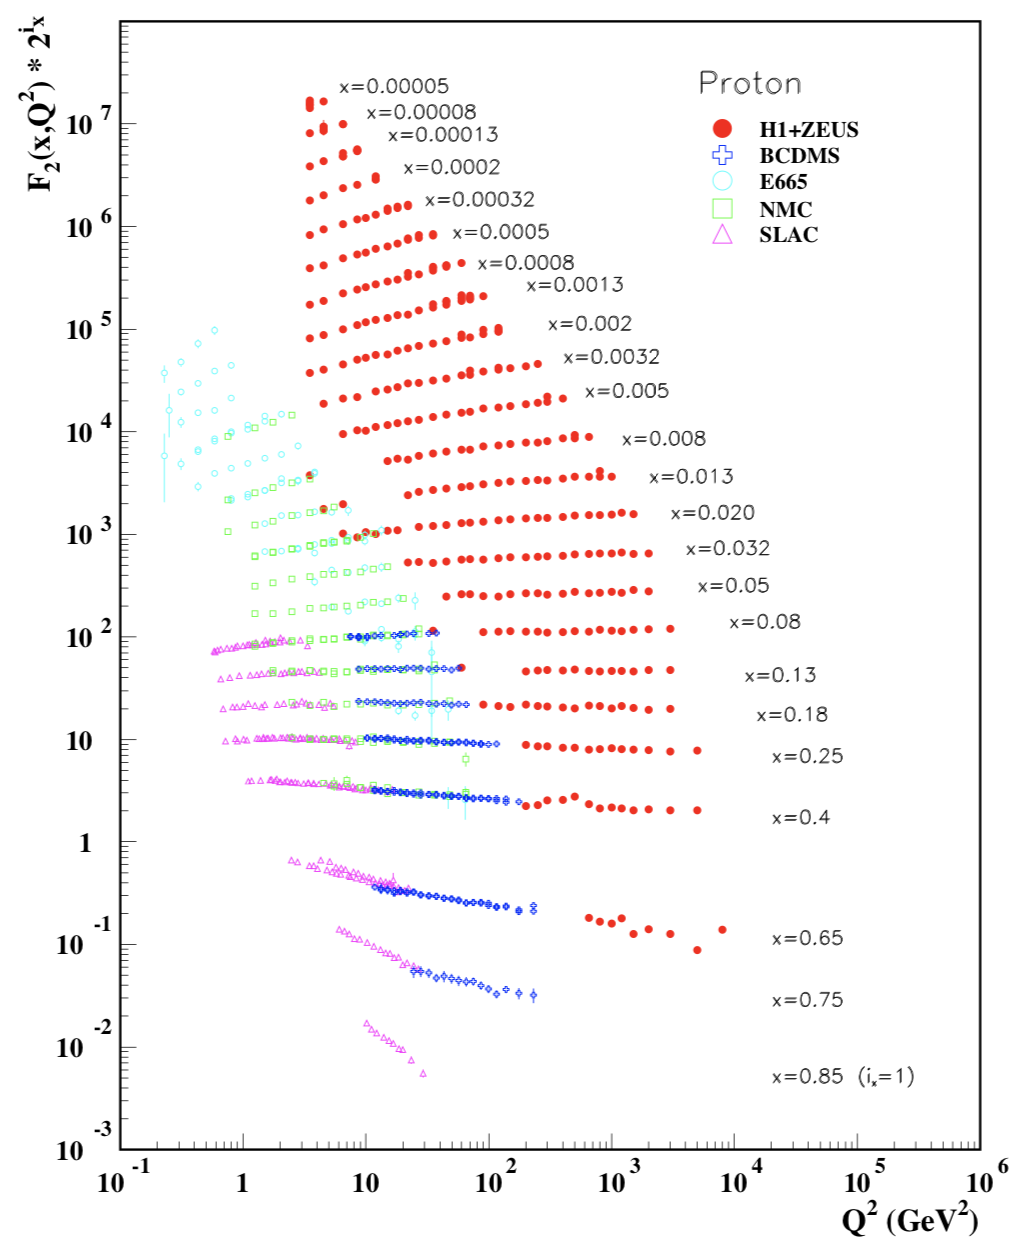
\includegraphics[scale=0.65]{./gfx/F2.png}
	\caption{The proton structure function $F^2_p$ measured in electromagnetic scattering of electrons and positrons on protons in the kinematic domain of the HERA data (collider experiments H$1$ and ZEUS for $Q^2 \geq 2$ GeV$^2$), and for electrons (SLAC) and muons (BCDMS, E$665$, NMC) on a fixed target. Figure taken from \cite{PDG}.}
	\label{pic:F2}
\end{figure}

\subsection{QCD-improved QPM}

The $Q^2$ dependence mentionned in previous subsection can be estimated by introducing quark interactions in the framework of QCD \cite{DISmeas,PICH}. Quantum ChromoDynamics is a non-abelian gauge theory based on a symmetry group SU($3$), which describes the interaction of quarks and gluons. The charge of this theory is called colour and the force carriers are the gluons, which are also coloured particles. The internal nucleon dynamic is due to the gluon emission and absorption and quark-antiquark pair creation from gluons. This creates a cloud of gluons and virtual $q\bar{q}$ pairs known as sea quarks.

The QCD coupling constant $\alpha_s$ depends on the scale of the interaction. At low energies quarks or gluons are always forming colorless particles, which are named hadrons: this is called confinement. At high energies quarks or gluons are free particles: this is asymptotic freedom.

Depending on the energy regime, a process can be labeled as a hard ($\alpha_s \sim 0$) or soft process ($\alpha_s large$). Hard processes can be described within the perturbative QCD (pQCD) framework, while soft processes can only be parametrized from experimental data. As in DIS the scale variable is often chosen as $Q^2$, the DIS cross-section is factorized \cite{CollinsSoper} in terms of soft and hard processes for $Q^2 > 1$ GeV$^2$, where $\alpha_s$ is small enough: the hard process is described by the lepton-quark cross-section $\sigma_q$ convoluted with the soft process parametrized by the PDFs. These two regimes differ by the factorisation scale $\Lambda$ that is mostly chosen as $Q^2$.

The resolution of the virtual photon probe is proportional to $1/Q^2$ (see Fig.~\ref{pic:Q2res} at fixed $x$). At $Q^2 \sim 0$, the virtual photon sees the nucleon as a point-like particle. As $Q^2$ increases, the virtual photon starts to resolve the nucleons constituents. At large $Q^2$ the virtual photon is able to resolve point-like quarks. The first QCD correction to the QPM concerns the gluon emission by the initial and the final quark.

\begin{figure}[!h]
  \centering
	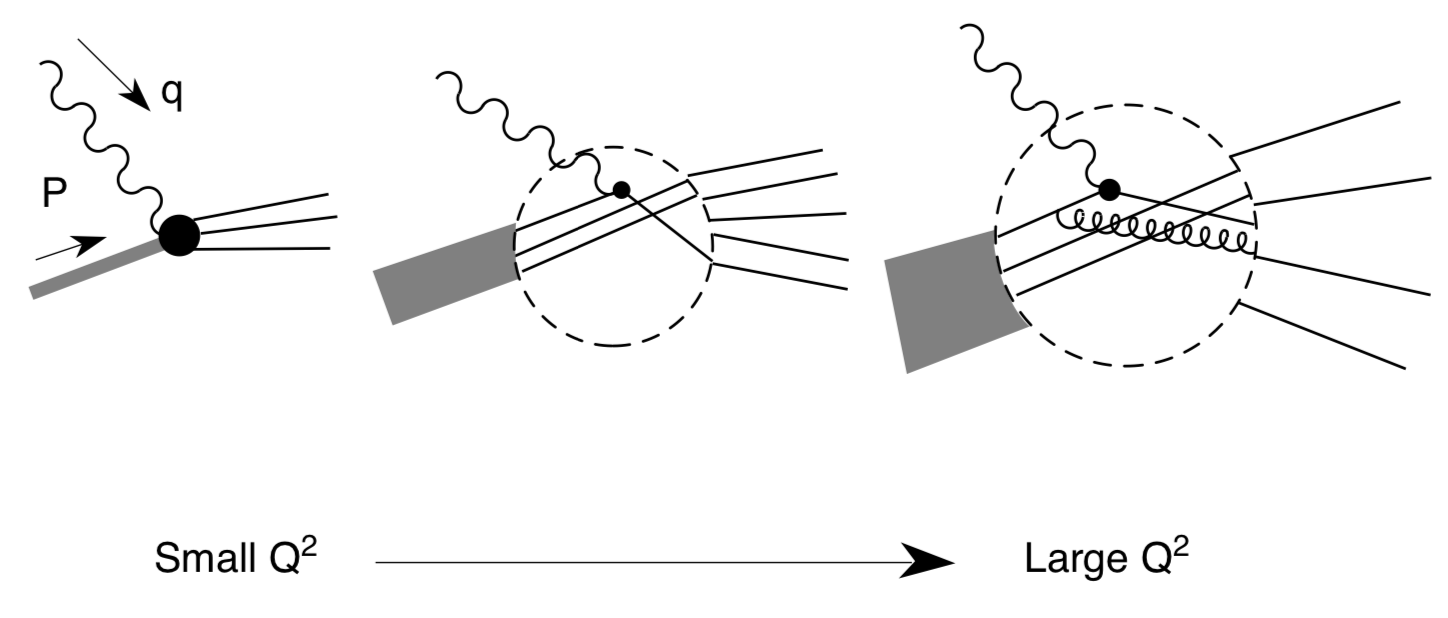
\includegraphics[scale=0.6]{./gfx/Q2res.png}
	\caption{Resolution of the photon probe versus $Q^2$. Figure taken from \cite{PICH}.}
	\label{pic:Q2res}
\end{figure}

The $Q^2$ dependence can be calculated using the Dokshiter-Gribov-Lipatov-Altarelli-Parisi (DGLAP) equations \cite{Dokshitser, GL1, GL2, AP}:
%
\begin{equation}
  \frac{dq_i(x,Q^2)}{dlnQ^2} = \frac{\alpha_s(Q^2)}{2\pi}\sum\limits_{j}\int_{x}^{1}P_{ij}(x/\xi,\alpha_s(Q^2))q_i(\xi,Q^2).
\end{equation}
%
Here, the splitting functions $P_{ij}(x/\xi)$ \cite{Joosten} are the probability that a quark or gluon of type $j$ and momentum fraction $\xi$ is the parent of $i$ with momentum fraction $x$. A similar equation holds for the gluon distribution. If the PDFs are known at a given scale $Q_0^2$, they can be evolved to any given $Q^2$ using these equations.

%----------------------------------------------------------------------------------------

\section{Determination of Parton Distribution Functions}

The PDFs are non-perturbative quantities and thus cannot be calculated from a theoretical framework. A global fit to world data is the only way to quantify them. It is possible to fit measurement coming from different processes because PDFs are universal quantities, i.e. they are process independent. The world data consists mostly of lepton-nucleon DIS but collider experiments ($pp$ or $p\bar{p}$) or neutrino scattering can be used for special contributions, e.g. for gluons or strange quarks. As experiments cover different kinematic ranges, this allows one to determine the PDFs in a large ($x$,$Q^2$) space.

For the fit to be performed, a functional form has to be provided at an initial scale $Q^2_0$. Often the form $xq_i(x,Q^2_0) = x^{\alpha}(1-x)^{\beta}$, where $q_i$ are partons, is used with additional terms refining the fit, reaching a number of free parameters from $10$ to $25$. The DGLAP equations are then used to evolve the PDFs to a given $Q^2$. An example of a fit done by the MMHT group \cite{MMHT} at Next to Leading Order (NLO) for different $Q^2$ values is shown in Fig.~\ref{fig:MMHT}.

\begin{figure}[htb!]
\centerline{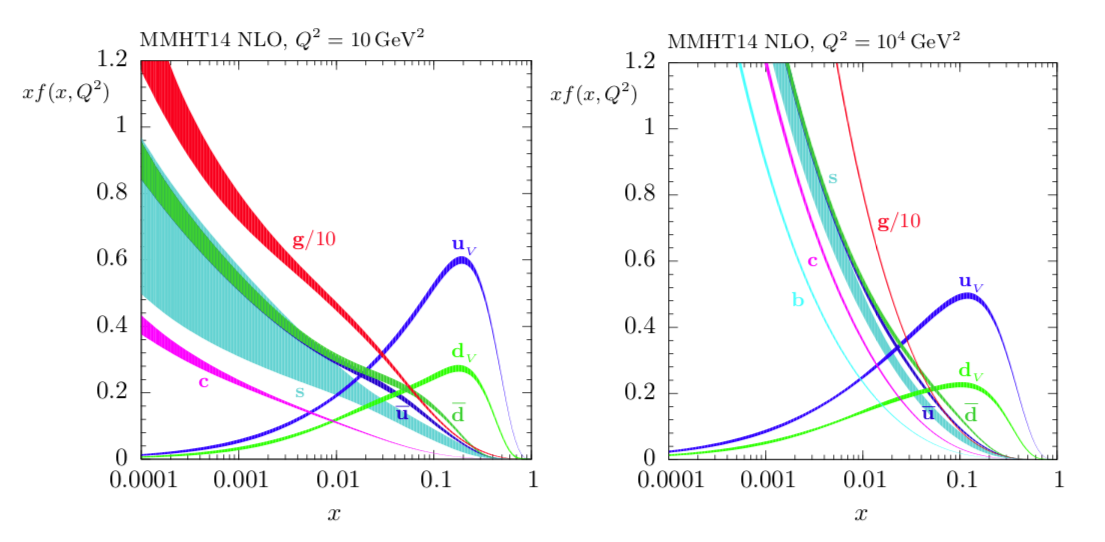
\epsfig{file=gfx/MMHT.png,width=14cm}}
\caption{Unpolarized PDFs at Next to Leading Order (NLO) from MMHT group at $Q^2$ = $10$ GeV$^2$ (left) and $Q^2$ = $10^4$ GeV$^2$ (right) with associated 68\% confidence-level uncertainty bands. Figure taken from \cite{MMHT}.}\label{fig:MMHT}
\end{figure}

%----------------------------------------------------------------------------------------

\section{Semi-Inclusive Deep Inelastic Scattering}

SIDIS is the semi-inclusive measurement of DIS. In the final state, at least one hadron and the scattered lepton are detected ($l+N \rightarrow l'+h+X$) and a new invariant variable $z$ is introduced, which corresponds to the energy fraction of the virtual photon held by the hadron $h$:
%
\begin{equation}
  z = \frac{\textbf{P}\cdot\textbf{p}_h}{\textbf{P}\cdot\textbf{q}} \stackrel{lab}{=} \frac{E_h}{\nu}.
  \label{eq:SIDIS}
\end{equation}
%
The semi-inclusive cross section reads \cite{SIDISXS}:
%
\begin{equation}
  \frac{d\sigma}{dxdydz} = \frac{8\pi\alpha^2ME}{Q^4}\left[xy^2H_1(x,Q^2,z)+(1-y)H_2(x,Q^2,z)\right],
  \label{eq:SIDISXS}
\end{equation}
%
where $H_1$ and $H_2$ are structure functions related to $F_1$ and $F_2$ \cite{BERGER,SIDISXS}:
%
\begin{equation}
  \sum\limits_{h}\int_{0}^{1} H_i(x,Q^2,z)dz = F_i(x,Q^2)\quad,\quad i \in  \llbracket1,2\rrbracket.
\end{equation}
%
Additional variables used to describe the hadron kinematics are given in Table.~\ref{tab:SIDIS}.

\begin{table}[h!]
  \caption{SIDIS kinematic variables.}
  \label{tab:SIDIS}
  \begin{tabularx}{\textwidth}{r|lX}
    \hline
    \hline
    Variable & Description \\
    \hline
    \hline
    $\textbf{p}=(E_h,\vec{p}_h)$ & Hadron $4$-momentum vector \\
    $p_{h\|}$ & Component of $\vec{p}_h$ along $\vec{q}$ \\
    $p_{h\bot}$ & Transverse component of $\vec{p}_h$ with respect to $\vec{q}$ \\
    $\theta_h$ & Angle between $\vec{q}$ and $\vec{p}_h$ \\
    $\Phi_h$ & Angle between the scattering plane and the hadron production plane \\
    $z=\frac{E_h}{\nu}$ & Energy fraction of the virtual photon transferred to the hadron $h$ \\
    $\eta=\frac{1}{2}\text{ln}\left(\frac{|\mathbf{p}|+p_L}{|\mathbf{p}|-p_L} \right)$ & Pseudorapidity \\
    \hline
    \hline
  \end{tabularx}
\end{table}

\subsection{SIDIS in QPM}

The factorization Ansatz is also valid for SIDIS measurement thus the hadron production can be described as a convolution of three independent processes: the soft part $q(x)$ that are the PDFs, the hard process $\sigma_q$ describing the absorption of the virtual photon $\gamma^*$ by the quark $q$ and the soft part $D_q^h(z)$ characterize the fragmentation of the quark $q$ into a hadron $h$.

\begin{figure}[!h]
  \centering
	% 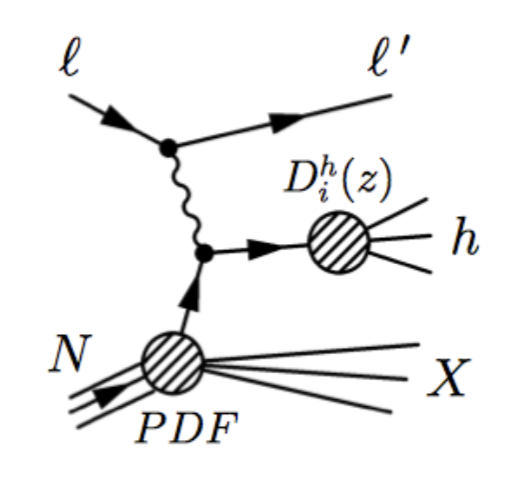
\includegraphics[scale=0.6]{./gfx/SIDIS.png}
  \begin{tikzpicture} \begin{feynman}
  \vertex (i1) {\(l\)};
  \vertex[right=2cm of i1] (a);
  \vertex[above right=2cm of a] (i2) {\(l'\)};
  \vertex[blob,below=2cm of a] (b) {\(\sigma_q\)};
  \vertex[blob,below left=2cm of b] (c) {\(q(x)\)};
  \vertex[below left=2cm of c] (f12) {\(N\)};
  \vertex[right=2cm of c] (f22);
  \vertex[below=0.3cm of f22] (f23);
  \vertex[above=0.3cm of f22] (f21);
  \vertex[blob, right=of b] (d) {\(D^h_q(z)\)};
  \vertex[above right=of d] (d1) {\(h^{\pm}\)};
  \vertex[right=of d] (d2) {\(\pi^{\pm}\)};
  \vertex[below right=of d] (d3) {\(K^{\pm}\)};

  \diagram* { (i1) -- [fermion] (a) -- [fermion] (i2),
  (a) -- [photon, edge label=\(\gamma^*\)] (b) [blob],
  (c) [blob] -- [fermion] (b) [blob],
  (b) [blob] -- [fermion] (d) [blob],
  (f12) -- [double distance=7pt] (c) [blob] -- [plain] (f22),
  (f12) -- [fermion] (c) [blob],
  (c) [blob] -- [plain] (f21),
  (c) [blob] -- [plain] (f23),
  (d) [blob] -- [plain] (d1),
  (d) [blob] -- [plain] (d2),
  (d) [blob] -- [plain] (d3),
  };
  \draw [decoration={brace}, decorate] (f21.north east) -- (f23.south east) node [pos=0.5, right] {\(X\)};
  \end{feynman} \end{tikzpicture}
	\caption{Factorization in SIDIS.}
	\label{pic:SIDIS}
\end{figure}

The structure functions $H_i(x,Q^2,z)$ contain the information on what happens to the struck quark after the interaction with the virtual photon. The fragmentation function (FF) $D_q^h(z,Q^2)$ is defined as the probability for a quark of flavour $q$ to fragment into a hadron $h$ with a fraction of energy $z$. The expression of the spin averaged SIDIS cross section can be expressed within QPM at LO in terms of PDFs and FFs \cite{BERGER,Panknin}:
%
\begin{equation}
  \frac{d^3 \sigma}{dxdydz} \stackrel{LO}{=} \frac{8\pi\alpha^2ME}{Q^2}\left[\frac{1}{2}y^2+\left(1-y-\frac{y^2 \gamma^2}{4}\right)\right]x\sum\limits_qe^2_qq(x)D_q^h(z).
  \label{eq:unpolSIDIS}
\end{equation}

%----------------------------------------------------------------------------------------

\section{Fragmentation Functions}\label{sec:FF}

When computing the cross-section of a given process $A+B \rightarrow h+X$, this cross-section is found to be a convolution of three different terms (Eq.~\ref{eq:facto}): one non-perturbative term involving the PDFs (probability to obtain parton $a$ from nucleus $A$ $f_{a/A}(x_a,Q^2)$), one hard cross-section term for perturbative calculation ($d\sigma_{a,b \rightarrow c}(x_a,x_b,Q^2)$) and a last non-perturbative term involving the FFs (probability to obtain hadron $h$ from parton $c$ $D^h_c(x_c,Q^2)$).
%
\begin{equation}
  d\sigma_{A+B \rightarrow h+X} = \sum_{a,b,c} \left[ f_{a/A}(x_a,Q^2) f_{b/B}(x_b,Q^2) \right] \otimes \left[ d\sigma_{a,b \rightarrow c}(x_a,x_b,Q^2) \right] \otimes \left[ D^h_c(x_c,Q^2) \right]
  \label{eq:facto}
\end{equation}
%
Fig.~\ref{pic:SIDIS} illustrates this factorization in SIDIS. The extraction of FFs can also be done from electron-positron annihilation and hadron-hadron collisions measurements. The universality of FFs has been experimentally tested by Kniehl, Kramer and Pötter \cite{Universality}. Different ideas have been developed to model how quarks confine together to make a hadron.

\subsection{Lund String Fragmentation Model}

In the Lund String Model \cite{LUND}, the hadron production is explained by the creation of quark-antiquark pairs $q\bar{q}$. The strong interaction between partons is represented by a string. The energy inside the string is linear function of the distance between two stringed partons. At some point the energy is large enough to create a new $q\bar{q}$ pair and the string breaks. All unpaired remnants have new strings and the process repeats until there are only hadrons. The hadronization scheme in the Lund model in the center of mass frame is illustrated in Fig.~\ref{pic:Lund} (a). The virtual photon is absorbed e.g. by a $u$ quark and in consequence the $u$ quark is ejected from the nucleon. A new $q\bar{q}$ pair is created by the string breaking e.g. $d\bar{d}$. The remaining $u$ quark binds with the $\bar{d}$ quark to form a $\pi^+$ with a given $z$ as shown in Fig.~\ref{pic:Lund} (b). The remaining system repeats fragmentation process until the energy is smaller than the available energy $\nu$. In addition baryon creation by di-$q\bar{q}$ pair formation is introduced.

\begin{figure}[!h]
  \centering
	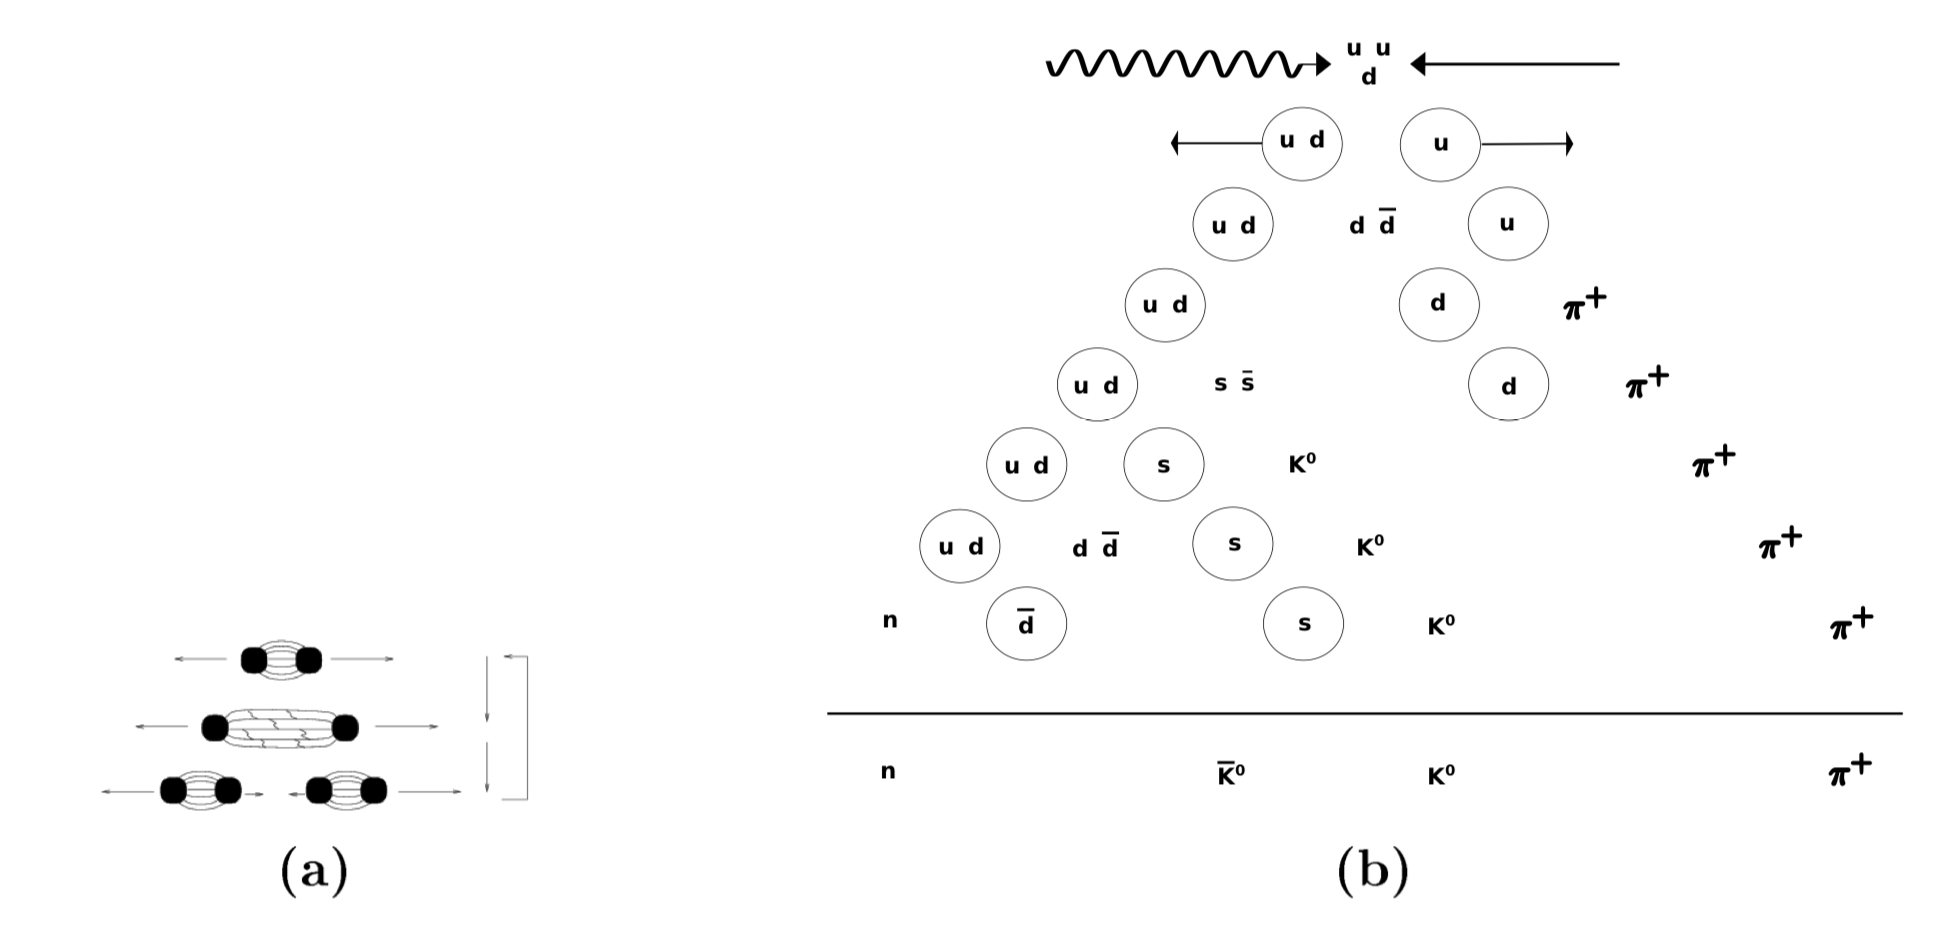
\includegraphics[scale=0.45]{./gfx/Lund.png}
	\caption{The fragmentation process in the Lund model. In (b), the produced $K^0$, $\overline{K^0}$, $\pi^+$ or $n$ could also be an excited state. Figure taken from \cite{Panknin}.}
	\label{pic:Lund}
\end{figure}

\subsection{Quark Fragmentation Regions}

Up to this point only the fragmentation of the struck quark was considered. The spectator quarks, which are not involved in the scattering process, have also to hadronize. This phenomenon is happening in two distinct $p_h$ regions: the target fragmentation region, where the final hadron $h$ has a small momentum in the rest frame of the target, and the current fragmentation region, where the product $\textbf{P}\cdot\textbf{p}_h$ grows with $Q^2$. At low energies there is a large overlap of these regions, while at high energies they start to separate. This hadron production can contaminate the SIDIS measurement of current fragmentation. To deal with this issue, Berger \cite{BERGER} came with a criterion based on the pseudorapidity of the final state $\eta$, which is the measurement of the longitudinal momentum. The sign of $\eta$ is linked to the different regions: if $\eta$ $>$ $0$ the hadron moves towards the direction of the virtual photon and is a current hadron, else is $\eta$ $<$ $0$ the hadron is a target remnant (Fig.~\ref{pic:Berger}). Defining $p(k)$ to be the probability that $k$ hadrons of some specific type decay from one cluster, one finds that the \textit{fully inclusive} correlation function has the form:
%
\begin{equation}
  C(y_1,y_2) = \frac{\langle k(k-1) \rangle}{\langle k \rangle} \left(\frac{1}{\sigma}\frac{d\sigma}{dy}\right)_{y\sim 0} G(y_1-y_2),
\end{equation}
%
when $y_1$ and $y_2$ are in the central region and the averages are:
%
\begin{equation}
  \begin{split}
    \langle k \rangle = \sum kp(k) \\
    \langle k-1 \rangle = \sum k(k-1)p(k).
  \end{split}
\end{equation}
%
The Gaussian function:
%
\begin{equation}
  G(y_1-y_2) = \frac{1}{2\delta \sqrt{\pi}}exp\left[-\frac{\left(y_1-y_2\right)}{4\delta^2}\right],
\end{equation}
%
has an effective \textit{correlation length} of $2\delta$. As the typical hadronic correlation length in pseudorapidity is $\delta \sim 2$, a separation criterion, the Berger criterion, is that $\Delta\eta = \eta_{max}-\eta_{min} \geq 2\delta$ or in terms of DIS kinematics variables $W \gtrsim 7.4$ GeV. It is important to select the kinematic region so that selected hadrons are dominated by the struck quark fragmentation.

\begin{figure}[!h]
  \centering
	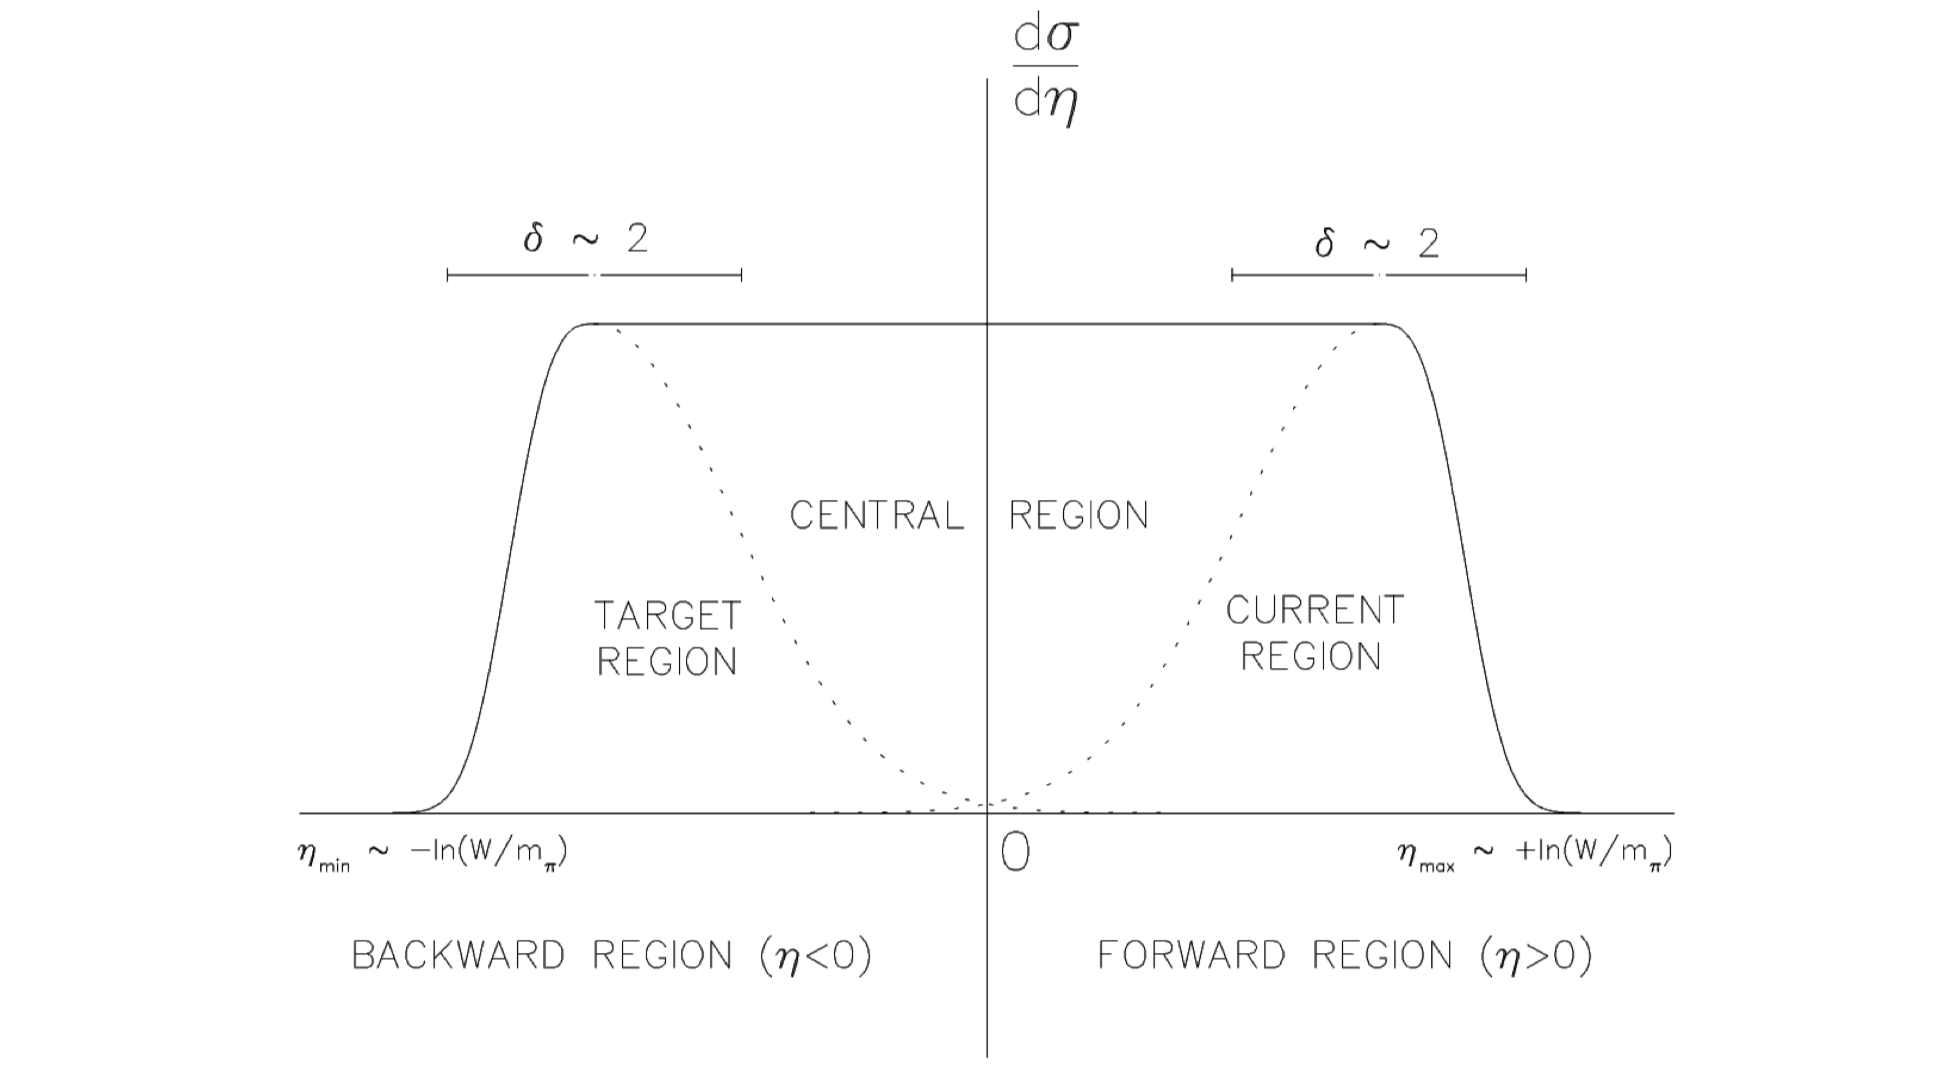
\includegraphics[scale=0.5]{./gfx/Berger.png}
	\caption{Hadronic pseudorapidity ($\eta$) distribution at very high energies. Figure taken from \cite{Niczy}.}
	\label{pic:Berger}
\end{figure}

\subsection{Scaling and $Q^2$ evolution}

For the FFs extracted from $e^+e^-$ annihilation displayed in Fig.~\ref{pic:FFscale}, the scaling is present for a wide $x = 2p_h/\sqrt{s}$ range (Fig.~\ref{pic:FFscale} (a)). At low x ($x$ $<$ $0.1$) the FFs increases with the total center-of-mass energy $\sqrt{s}$ (Fig.~\ref{pic:FFscale} (b)), while at large $x$, the FFs are shifted towards lower values for large $Q^2$ (similar behaviour as PDFs). Here $\sqrt{s}$ has the same role has $Q^2$. Scaling violation is observed \cite{PDG}.

\begin{figure}[!h]
  \centering
	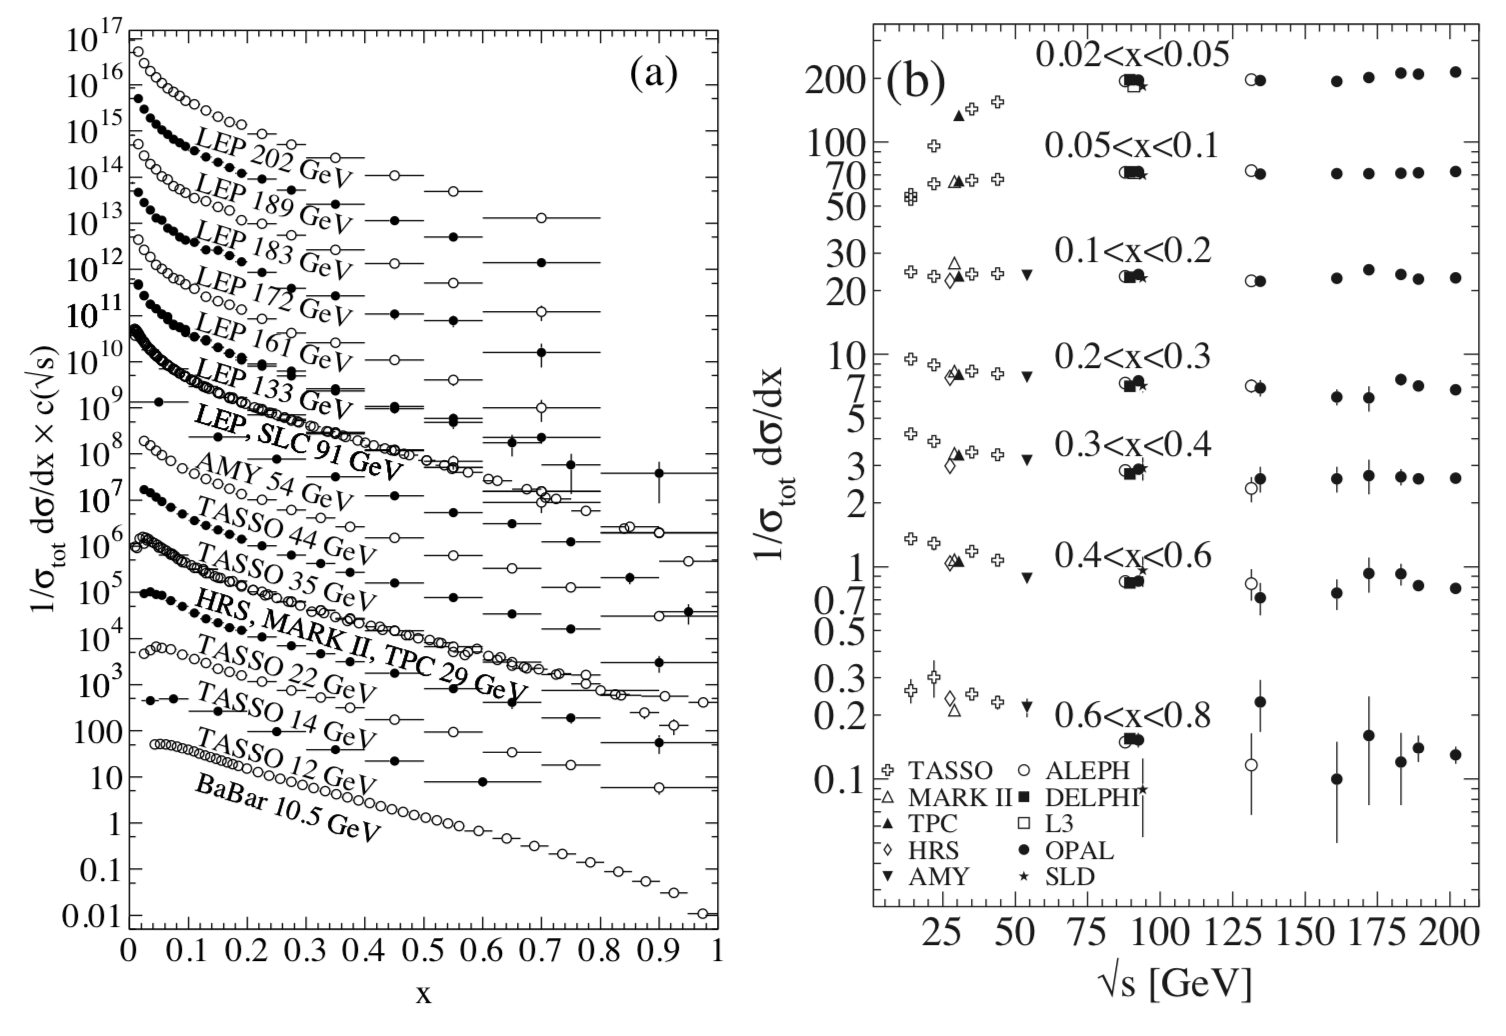
\includegraphics[scale=0.6]{./gfx/FFscale.png}
	\caption{The $e^+ e^-$ fragmentation function for all charged particles for different center of mass energy $\sqrt{s}$ versus $x$ (a) and for various range of $x$ versus $\sqrt{s}$ (b). Figures taken from \cite{PDG}.}
	\label{pic:FFscale}
\end{figure}

The evolution of the fragmentation functions is also described by DGLAP equations \cite{Dokshitser, GL1, GL2, AP}:
%
\begin{equation}
  \frac{dD_q^h(z,Q^2)}{dlnQ^2} = \frac{\alpha_s(Q^2)}{2\pi}\sum\limits_j\int_{x}^{1}P_{qj}\left(z/\xi,\alpha_s(Q^2)\right)D_q^h(\xi,Q^2)\frac{d\xi}{\xi}.
\end{equation}
%
In Fig.~\ref{pic:QuarkFrag} the process contributing to the $Q^2$-evolution is illustrated~: the fragmentation of a quark $q_i$ through its own hadronization after emmiting a gluon $G$ ($P_{qq}D_{q_i}^h$), through the hadronization of a gluon $G$ ($P_{Gq}D_{G}^h$), the fragmentation of a gluon splitting into a quark-antiquark pair and following hadronization of the quark in hadron ($P_{qG}D_{q_i}^h$) and eventually the gluon fragmentation via the three-gluon self-interaction ($P_{GG}D_{G}^h$).

\begin{figure}[!h]
  \centering
	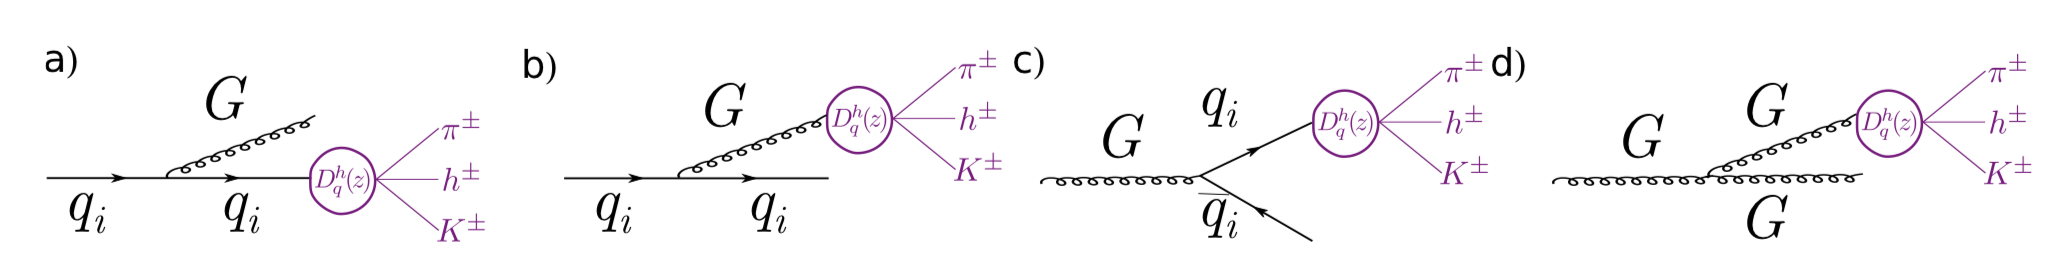
\includegraphics[scale=0.45]{./gfx/QuarkFrag.png}
	\caption{The fragmentation of the quark $q_i$ decaying into a hadron $h$ while emitting a gluon $G$ ($P_{qq}D^h_{q_{i}}$) (a), the fragmentation of the quark $q_i$ through a gluon $G$ ($P_{Gq}D^h_{G}$) (b), the fragmentation of the gluon $G$ via the creation of a $q_i \bar{q_i}$ pair and the decay of $q_i$ ($P_{qG}D^h_{q_{i}}$) (c) and the fragmentation of the gluon $G$ via a three gluon vertex ($P_{GG}D^h_{G}$) (d). Figure taken from \cite{Uematsu}.}
	\label{pic:QuarkFrag}
\end{figure}

\subsection{Fragmentation Function Symmetries}

One FF $D^h_q(z,Q^2)$ is introduced for each flavour $q$ and each hadron species $h$. Considering only the light quarks ($u$,$\bar{u}$,$d$,$\bar{d}$,$s$ and $\bar{s}$), in case the mass threshold for heavy quarks is higher than the covered kinematic domain, implies that for charged hadrons one has to measure twelve different fragmentation functions for positive and negative hadrons. Nevertheless, within the QCD-improved QPM, symmetries as isospin or charge-conjugation can be used to reduce the number of independent fragmentation functions.

The FFs can be split into two main categories. If a quark fragments into a hadron h and the quark is a valence quark of $h$, the FF is said to be favoured ($D^h_{fav}$). If it is a sea quark of $h$, the FF is unfavoured ($D^h_{unf}$).

For pions charge-conjugation symmetry reduces the number of independent fragmentation functions to six. The application of the isospin (viz. $D^{\pi^+}_u = D^{\pi^+}_{\bar{d}}$ for $\pi^+$) and SU($3$) symmetries lowers this number further to two:
%
\begin{equation}\label{eq:FFPion}
  \begin{split}
    D^h_{fav}: D^{\pi^+}_u = D^{\pi^-}_{\bar{u}} = D^{\pi^-}_d = D^{\pi^+}_{\bar{d}}, \\
    D^h_{unf}: D^{\pi^-}_u = D^{\pi^+}_{\bar{u}} = D^{\pi^+}_d = D^{\pi^-}_{\bar{d}} \stackrel{SU(3)\,sym.}{=} D^{\pi^{\pm}}_s = D^{\pi^{\mp}}_{\bar{s}}.
  \end{split}
\end{equation}

For kaons charge-conjugation symmetry reduces the number of independent fragmentation functions to six. The application of the isospin (viz. $D^{\pi^+}_u = D^{\pi^+}_{\bar{d}}$ for $\pi^+$) and SU($3$) symmetries lower the number to three independent FFs: the favoured, grouping the kaons valence quarks $u$ and $\bar{u}$ FFs, the strange, grouping the kaons valence quarks $s$ and $\bar{s}$ FFs and the unfavoured, grouping the kaons sea quark FFs:
%
\begin{equation}\label{eq:FFKaon}
  \begin{split}
    D^h_{fav}: D^{K^+}_u = D^{K^-}_{\bar{u}} \\
    D^h_{str}: D^{K^+}_{\bar{s}} = D^{K^-}_{s} \\
    D^h_{unf}: D^{K^+}_{\bar{u}} = D^{K^-}_{u} = D^{K^+}_s = D^{K^-}_{\bar{s}} = D^{K^{\pm}}_{d} = D^{K^{\mp}}_{\bar{d}}
  \end{split}
\end{equation}

%----------------------------------------------------------------------------------------

\section{State of the art of the fragmentation functions}

\subsection{Measurements}

The production of hadrons from the the struck quark cannot be computed as final state hadron masses are of order or smaller than $\Lambda_{QCD}$. In order to extract FFs reliably from the $Q^2$ dependence of the measured hadron production, a large kinematic range is needed. Thus data taken at different energies are used. Three different processes are so far used to extract quark fragmentation functions: electron-positron annihilation (SIA), lepton-nucleon (SIDIS) and hadron-hadron collisions ($pp$ or $p\bar{p}$). A summary of the aspects of the different processes can be found in Table.~\ref{tab:FFProcesses}. The SIA data (LEP \cite{LEP1,LEP2,LEP3}, SLAC \cite{SLAC1}, BaBar \cite{BABAR} and BELLE \cite{BELLE}) provide the cleanest access to the FFs, since the cross-section of the process does not involve PDFs and are well calculated up to NNLO. But due to the dependence of the cross-section on $e^2_q$, $D^h_q$ and $D^h_{\bar{q}}$ cannot be separated and there is a limited access to gluon FF $D^h_g$. The data from hadron-hadron collisions (UA5 \cite{UA5}, UA1 \cite{UA1}, ALICE \cite{ALICE}, CMS \cite{CMS1,CMS2}, ATLAS \cite{ATLAS}, RHIC \cite{RHIC1,RHIC2,RHIC3}) give access to $D^h_q$, $D^h_{\bar{q}}$ and $D^h_g$, but allow no direct access to $z$.

Data from SIDIS can be compared to data from previously presented processes for the current fragmentation region (see Section~\ref{sec:FF}). SIDIS data have the advantage that factorization has been proven to all orders of $\alpha_s$. In addition they cover a wide range in $Q^2$ in a single measurement compared to SIA. The experiments providing inputs for the SIDIS process are EMC \cite{EMC} and COMPASS \cite{COMPASS2006Pi,COMPASS2006K} using muon beam and E$00$-$108$ \cite{E00108} and HERMES \cite{HERMESMult} using electron beam. All experiments measured with proton and deuteron targets.

\begin{table}[!h]
  \caption{Fragmentation functions access for different processes.}
  \label{tab:FFProcesses}
  \centering
  \begin{tabular}{cccc}
    \hline
    \hline
    & $e^+ e^- annihilation$ & $pp$/$p\bar{p}$ collision & DIS \\
    \hline
     &   \resizebox{3cm}{3.5cm}{\begin{tikzpicture} \begin{feynman}
     \vertex (i1) {\(e^{-}\)};
     \vertex[right=2cm of i1] (a);
     \vertex[above right=2cm of a] (i2) {\(e^{+}\)};
     \vertex[blob,below=2cm of a] (b) {\(\widehat{\sigma_q}\)};
     \vertex[below left=2cm of b] (f12);
     \vertex[below=0.3cm of f12] (f13);
     \vertex[above=0.3cm of f12] (f11);
     \vertex[blob,below right=2cm of b] (d) {\(D^h_q(z)\)};
     \vertex[above right=of d] (d1) {\(h^{\pm}\)};
     \vertex[right=of d] (d2) {\(\pi^{\pm}\)};
     \vertex[below right=of d] (d3) {\(K^{\pm}\)};

     \diagram* { (i1) -- [fermion] (a) -- [anti fermion] (i2),
     (a) -- [photon, edge label=\(\gamma^{*}/Z^{0}\)] (b) [blob],
     (f12) -- [plain] (b) [blob] -- [fermion] (d) [blob],
     (f13) -- [plain] (b) [blob],
     (f11) -- [plain] (b) [blob],
     (d) [blob] -- [plain] (d1),
     (d) [blob] -- [plain] (d2),
     (d) [blob] -- [plain] (d3),
     };
     \draw [decoration={brace}, decorate] (f13.south west) -- (f11.north west) node [pos=0.5, left] {\(X\)};
   \end{feynman} \end{tikzpicture}}
      & \resizebox{3.5cm}{3cm}{\begin{tikzpicture} \begin{feynman}
    \vertex (i1) {\(p\)};
    \vertex[blob,right=2cm of i1] (a) {\(q(x)\)};
    \vertex[below=6cm of i1] (i2) {\(p/\bar{p}\)};
    \vertex[blob,right=2cm of i2] (b) {\(q(x)\)};
    \vertex[blob,below right=4cm of a] (c) {\(\widehat{\sigma}_q\)};
    \vertex[above right=of c] (f1);
    \vertex[blob, below right=of c] (d) {\(D^h_q(z)\)};
    \vertex[above right=of d] (d1) {\(h^{\pm}\)};
    \vertex[right=of d] (d2) {\(\pi^{\pm}\)};
    \vertex[below right=of d] (d3) {\(K^{\pm}\)};

    \diagram* { (i1) -- [double distance=7pt] (a) [blob], (i1) -- [fermion] (a) [blob],
    (i2) -- [double distance=7pt] (b) [blob], (i2) -- [fermion] (b) [blob],
    (a) -- [fermion] (c) [blob], (b) -- [fermion] (c) [blob], (c) [blob] -- [fermion] (f1), (c) [blob] -- [fermion, edge label=\(q\)] (d) [blob],
    (d) [blob] -- [plain] (d1),
    (d) [blob] -- [plain] (d2),
    (d) [blob] -- [plain] (d3),
    };
    \end{feynman} \end{tikzpicture}}
      & \resizebox{3cm}{3.5cm}{\begin{tikzpicture} \begin{feynman}
      \vertex (i1) {\(l\)};
      \vertex[right=2cm of i1] (a);
      \vertex[above right=2cm of a] (i2) {\(l'\)};
      \vertex[blob,below=2cm of a] (b) {\(\widehat{\sigma}_q\)};
      \vertex[blob,below left=2cm of b] (c) {\(q(x)\)};
      \vertex[below left=2cm of c] (f12) {\(N\)};
      \vertex[right=2cm of c] (f22);
      \vertex[below=0.3cm of f22] (f23);
      \vertex[above=0.3cm of f22] (f21);
      \vertex[blob, right=of b] (d) {\(D^h_q(z)\)};
      \vertex[above right=of d] (d1) {\(h^{\pm}\)};
      \vertex[right=of d] (d2) {\(\pi^{\pm}\)};
      \vertex[below right=of d] (d3) {\(K^{\pm}\)};

      \diagram* { (i1) -- [fermion] (a) -- [fermion] (i2),
      (a) -- [photon, edge label=\(\gamma^*\)] (b) [blob],
      (c) [blob] -- [fermion] (b) [blob],
      (b) [blob] -- [fermion] (d) [blob],
      (f12) -- [double distance=7pt] (c) [blob] -- [plain] (f22),
      (f12) -- [fermion] (c) [blob],
      (c) [blob] -- [plain] (f21),
      (c) [blob] -- [plain] (f23),
      (d) [blob] -- [plain] (d1),
      (d) [blob] -- [plain] (d2),
      (d) [blob] -- [plain] (d3),
      };
      \draw [decoration={brace}, decorate] (f21.north east) -- (f23.south east) node [pos=0.5, right] {\(X\)};
    \end{feynman} \end{tikzpicture}}\\
    Dependence & $\widehat{\sigma} \otimes FF$ & $\widehat{\sigma} \otimes PDF \otimes PDF \otimes FF$ & $\widehat{\sigma} \otimes PDF \otimes FF$ \\
    Separate $D^h_{q}$ / $D^h_{\bar{q}}$ & \ding{55} & \ding{51} & \ding{51} \\
    Access parton kinematics & \ding{51} & \ding{55} & \ding{51} \\
    Theoretical calculation & LO, NLO, NNLO & LO, NLO & LO, NLO \\
    \hline
  \end{tabular}
\end{table}

\subsection{Accessing the fragmentation functions in SIDIS}

Hadron multiplicities are defined as the cross-section ratio:
%
\begin{equation}
  M^h(x,Q^2,z) = \frac{d\sigma^{lN \rightarrow l'hX}}{d\sigma^{lN \rightarrow l'X}dz} = \frac{d\sigma^h(x,Q^2,z)/dxdQ^2dz}{d\sigma^{DIS}(x,Q^2)/dxdQ^2},
\end{equation}
%
equivalent to the number of hadrons produced per DIS events allowing to access FFs by measuring hadron multiplicities.

Using the expressions of the DIS and SIDIS cross-sections (Eqs.~\ref{eq:unpolDIS} and \ref{eq:unpolSIDIS}) one obtains in the QPM:
%
\begin{equation}\label{eq:MFFPDF}
  M^h(x,Q^2,z) = \frac{\sum_q e^2_q q(x,Q^2) \otimes D^h_q(z,Q^2)}{\sum_q e^2_q q(x,Q^2)} \stackrel{LO}{=} \frac{\sum_q e^2_q q(x,Q^2) D^h_q(z,Q^2)}{\sum_q e^2_q q(x,Q^2)}.
\end{equation}
%
As PDFs and FFs depend on different variables $x$ and $z$ one can write the convolution as a single product. By measuring $M^h(x,Q^2,z)$ for positive and negative hadrons, one can distinguish $D^h_q$ and $D^h_{\bar{q}}$. The procedure of FFs extraction from COMPASS multiplicity measurement is described in Chapter~\ref{ch:FF}.

\subsection{Global fits of multiplicity data and parametrizations of FFs}

As the FFs are universal quantities, a global QCD fit of available data on multiplicities from SIA, SIDIS and $pp$/$p\bar{p}$ collisions can be performed to give a general parametrization of the FFs. There are different parametrization available in the literature. Some parametrizations are only based on SIA data: KKP \cite{Universality}, KRE \cite{KRE} and HKNS \cite{HKNS}, when the AKK \cite{AKK} parametrization uses in addition some hadron-hadron scattering data. One only uses SIDIS data: LSS \cite{LSS}. The newest parametrizations from DSEHS \cite{DSEHS1,DSEHS2} include all three types of data and JAM \cite{JAM} parametrizations include SIA+SIDIS. Each parametrization has its own set of assumptions based on symmetries and its different parametrization of $D^h_q$. A summary of the assumptions of the different groups can be found in Table \ref{tab:FFParametrization}. Only DSEHS and JAM will be described in more details in the following as they are the latest ones (or have been updated recently).

\begin{table}[!h]
  \caption{Parametrization of FFs for pions and kaons.}
  \label{tab:FFParametrization}
  \centering
  \begin{tabular}{ccccccc}
    \hline
    \hline
    Parametrization & Year & \multicolumn{3}{c}{Data} & \multicolumn{2}{c}{\# FFs fitted} \\
    \hline
     & & SIDIS & $pp$/$p\bar{p}$ & SIA & $\pi$ & $K$ \\
    KKP \cite{Universality} & 2000 & \ding{55} & \ding{55} & \ding{51} & 5 & 5 \\
    KRE \cite{KRE} & 2001 & \ding{51} & \ding{55} & \ding{51} & 2 & 3 \\
    HKNS \cite{HKNS} & 2007 & \ding{55} & \ding{55} & \ding{51} & 2 & 2 \\
    AKK \cite{AKK} & 2008 & \ding{55} & \ding{51} & \ding{51} & 3 & 5 \\
    LSS \cite{LSS} & 2014 & \ding{51} & \ding{55} & \ding{55} & 3 & 3 \\
    DSEHS \cite{DSEHS1,DSEHS2} & 2017 & \ding{51} & \ding{51} & \ding{51} & 4 & 4 \\
    JAM \cite{JAM} & 2018 & \ding{51} & \ding{55} & \ding{51} & 3 & 3 \\
    \hline
  \end{tabular}
\end{table}

\subsubsection*{DSEHS parametrization}

DSEHS (previously DSS) was the first group, who determined individual FFs for quarks and antiquarks and the first to try to fit data coming from three different processes alltogether.
The functional form they use for $D^h_q$ is the following:
%
\begin{equation}
  D^h_i (z,Q_0) = \frac{N^h_i z^{\alpha^h_i}(1-z)^{\beta^h_i}\left[ 1+\gamma^h_i(1-z)^{\delta^h_i}\right]}{B\left[2+\alpha^h_i,1+\beta^h_i\right]+\gamma^h_i B\left[2+\alpha^h_i,1+\beta^h_i+\delta^h_i\right]},
  \label{eq:DSEHSparam}
\end{equation}
%
where $N^h_i$, $\alpha^h_i$, $\beta^h_i$, $\gamma^h_i$ and $\delta^h_i$  are the fit parameters and B is the Euler beta function. For pions the two independent favoured FFs are related by a proportionality factor $k$. Moreover, isospin symmetry is considered only for the unfavoured FF ($D^{\pi^{+}}_{\bar{u}} = D^{\pi^{+}}_{d}$) and the fragmentation of a strange quark into pion is related to the unfavoured FFs with $z$-dependent factor ($D^{\pi^{+}}_{\bar{s}} = D^{\pi^{+}}_{s}=N_s z^{\alpha_s} D^{\pi^{+}}_{\bar{u}}$). Thus four FFs are fitted for pions: $u+\bar{u}$, $d=\bar{u}$, $s+\bar{s}$ and $g$. For kaons, $D^{K^+}_{u+\bar{u}}$ and $D^{K^+}_{s+\bar{s}}$ are fitted independently to account for the fact that phenomenologically it is expected that the formation of secondary $s\bar{s}$, required to form $K^+$ from a $u$, should be suppressed. Previous fits from DSS showed that $D^{K^+}_{s+\bar{s}} > D^{K^+}_{u+\bar{u}}$, highlighting this fact. For the unfavoured FFs all distributions have the same functional form  $D^{K^+}_{\bar{u}} = D^{K^+}_{s} = D^{K^+}_{d} = D^{K^+}_{\bar{d}}$ as the data are unable to discrimate between flavours. Four FFs are fitted for kaons, as for the pions:  $u+\bar{u}$, $s+\bar{s}$ , $\bar{u}=d=\bar{d}=s$ and $g$.
The FFs for heavy quarks (c,b) are also considered above their $\overline{MS}$ mass thresholds.
The parameters are determined from a standard $\chi^2$ minimization:
%
\begin{equation}
  \chi^2 =  \sum_{i=1}^{m} \left[ \left( \frac{1-\mathscr{N}_i}{\delta\mathscr{N_i}} \right) + \sum_{j=1}^{m_i} \frac{(\mathscr{N}_i T_j - E_j)^2}{\delta E^2_j} \right],
  \label{eq:DSEHSmin}
\end{equation}
%
where $m$ is the number of datasets with $m_i$ points each, $E_j$ are the data points and $\delta E_j$ their error and $T_j$ the theoretical estimate for a given set. The normalisation factor $\mathscr{N}_i$ is defined as $\delta \chi^2 / \delta\mathscr{N}_i = 0$.

\begin{table}[!h]
  \caption{DSEHS FFs hypotheses for pions and kaons.}
  \label{tab:DSEHSParametrization}
  \centering
  \begin{tabular}{ll}
    \hline
    \hline
     & Pions \\
    \hline
    Favoured & $D^{\pi^{+}}_{u} = N_{\pi^{+}} D^{\pi^{+}}_{\bar{d}}$ = $D^{\pi^{-}}_{d} = k_{\pi^{-}} D^{\pi^{-}}_{\bar{u}}$ \\
    Unfavoured & $D^{\pi^{+}}_{\bar{u}} = D^{\pi^{+}}_{d}$ \\
    Unfavoured strange & $D^{\pi^{+}}_{\bar{s}} = D^{\pi^{+}}_{s}$ \\
     & $D^{\pi^{-}}_{\bar{d}} = D^{\pi^{-}}_{u}$ = $D^{\pi^{-}}_{\bar{s}} = D^{\pi^{-}}_{s} = k_{\pi^{-}} D^{\pi^{-}}_{u}$ \\
    Gluons & $D^{\pi^{+}}_{g} = D^{\pi^{-}}_{g}$ \\
    \hline
    \hline
     & Kaons \\
    \hline
    Favoured & $D^{K^{+}}_{u}, D^{K^{-}}_{\bar{u}}$ \\
    Unfavoured & $D^{K^{+}}_{\bar{u}} = D^{K^{+}}_{d} = D^{K^{+}}_{\bar{d}} = D^{K^{+}}_{s}$ \\
               & $D^{K^{-}}_{u} = D^{K^{-}}_{d} = D^{K^{-}}_{\bar{d}} = D^{K^{-}}_{\bar{s}}$ \\
    Strange & $D^{K^{+}}_{\bar{s}}, D^{K^{-}}_{s}$ \\
    Gluons & $D^{K^{+}}_{g}, D^{K^{-}}_{g}$ \\
  \end{tabular}
\end{table}

The favoured, unfavoured and gluon FFs from DSS at LO for $Q^2$ = 10 GeV$^2$ are shown as function of $z$ for $\pi^+$ in Fig.~\ref{pic:DSEHSPi} and $K^+$ in Fig.~\ref{pic:DSEHSK}.

\begin{figure}[!h]
  \centering
	\includegraphics[scale=0.47]{./gfx/DSEHSPi.png}
	\caption{Individual FFs for positively charged pions $zD^{\pi^+}(z,Q^2)$ at $Q^2$ = $10$ GeV$^2$ (solid lines) along with uncertainty estimates at $68$\% and $90$\% C.L. indicated by the inner and outer shaded bands, respectively. The panels on the right-hand-side show the corresponding relative uncertainties. Also shown is a comparison to previous DSS$07$ global analysis \cite{DSS07} (dashed lines). Figure taken from \cite{DSEHS1}.}
	\label{pic:DSEHSPi}
\end{figure}

\begin{figure}[!h]
  \centering
	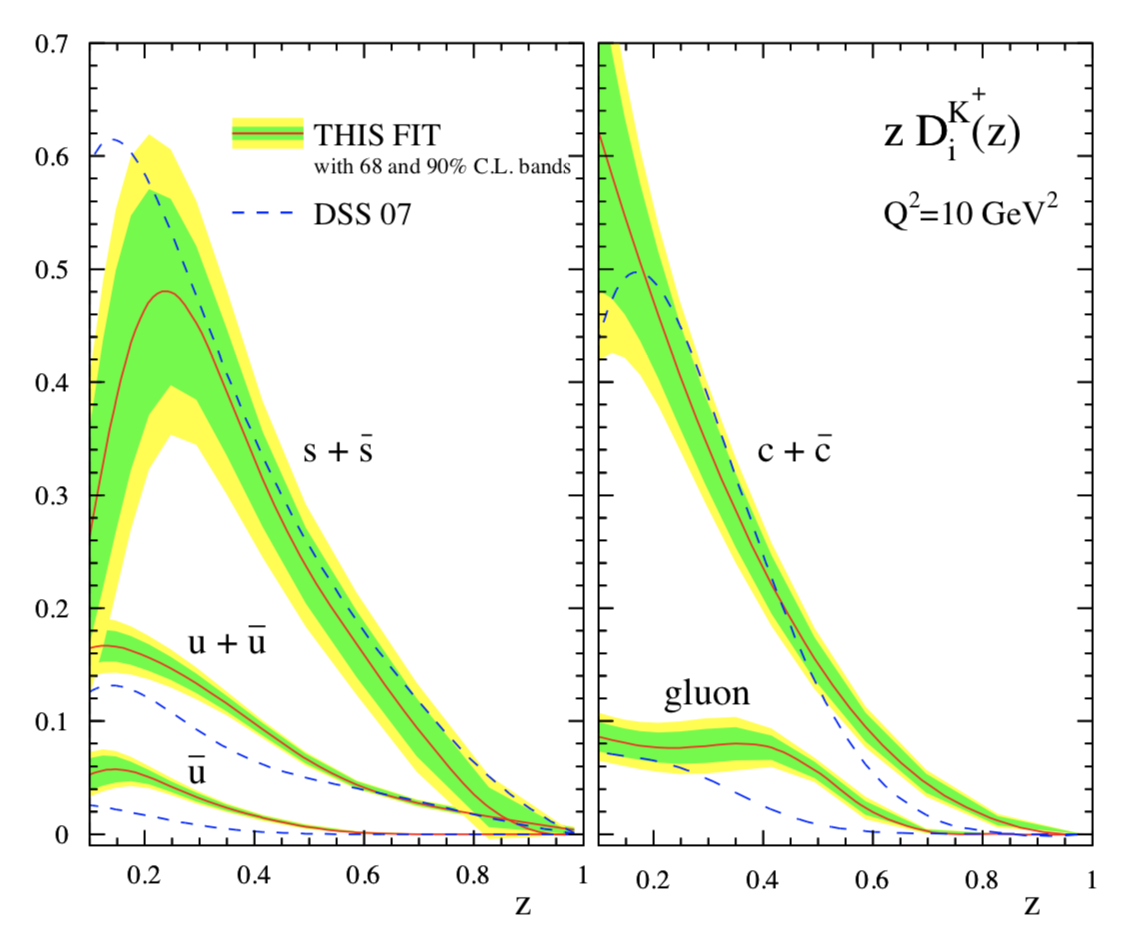
\includegraphics[scale=0.5]{./gfx/DSEHSK.png}
	\caption{Individual FFs for positively charged kaons $zD^{K^+}(z,Q^2)$ at $Q^2$ = $10$ GeV$^2$ (solid lines) along with uncertainty estimates at $68$\% and $90$\% C.L. indicated by the inner and outer shaded bands, respectively. Also shown is a comparison to previous DSS$07$ global analysis \cite{DSS07} (dashed lines). Figure taken from \cite{DSEHS2}.}
	\label{pic:DSEHSK}
\end{figure}

\subsubsection*{JAM parametrization}

JAM is a Monte-Carlo based combined fit of PDFs and FFs using Bayesian statistics. In order to address some of the questions raised by the recent ambiguities in the strange quark FFs and their impact on the $\Delta s$ determination, they go beyond the standard fitting paradigm by performing the first Monte Carlo (MC) analysis of PDFs and FFs, extending the methodology of the iterative Monte-Carlo (IMC) approach already used for the analysis of spin-dependent PDFs \cite{IMC} to the case of FFs (Fig.~\ref{pic:IMC}). The IMC approach allows for a full exploration of the parameter space using Monte-Carlo sampling together with data resampling techniques and cross validation of the fit. In consequence it reduces considerably any bias introduced by fine-tuning or fixing specific parameters that are not well constrained by the data.


\begin{figure}[!h]
  \centering
	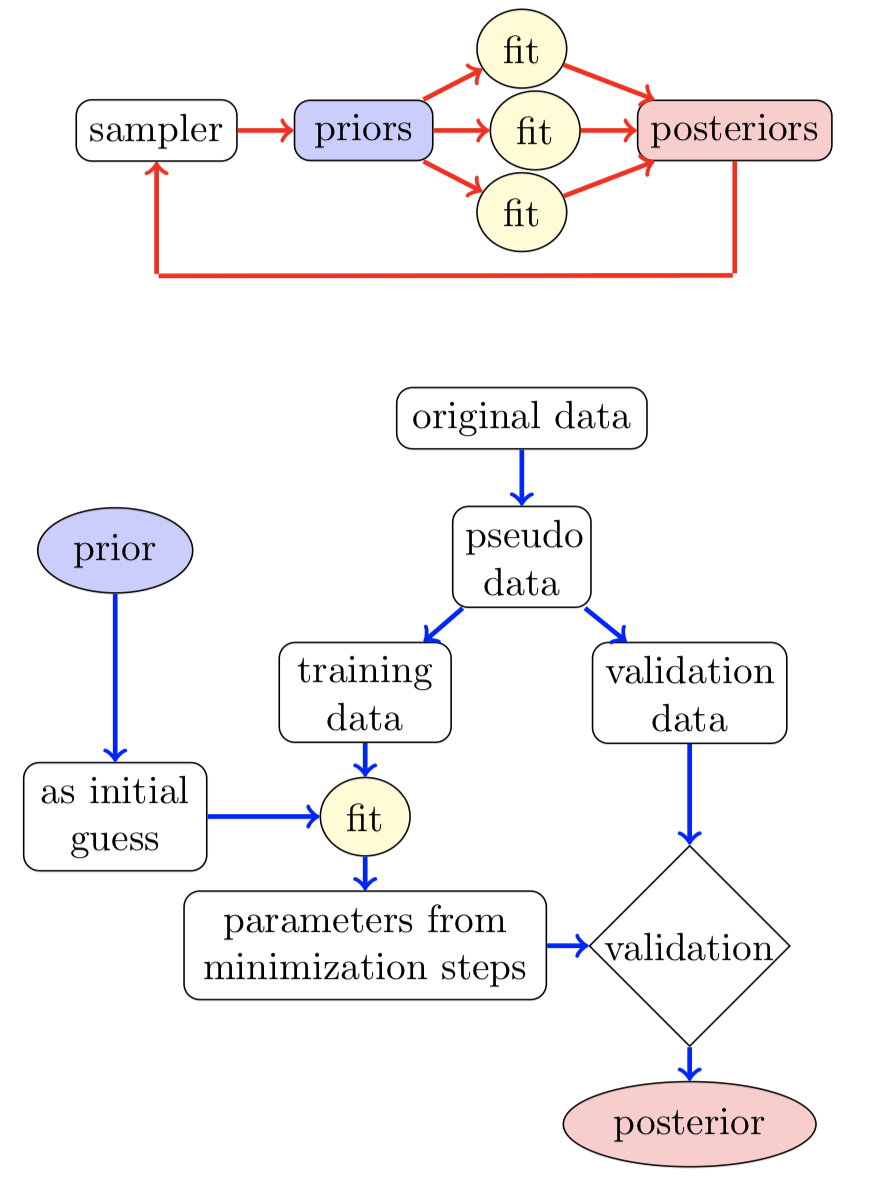
\includegraphics[scale=0.45]{./gfx/IMC.png}
	\caption{Workflow of the iterative Monte Carlo fitting strategy. In the upper diagram (red lines) an iteration begins at the prior sampler and a given number of fits are performed generating an ensemble of posteriors. After the initial iteration, with a flat sampler, the generated posteriors are used to construct a multivariate Gaussian sampler for the next iteration. The lower diagram (with blue lines) summarizes the workflow that transforms a given prior into a final posterior. Figure taken from \cite{IMC}.}
	\label{pic:IMC}
\end{figure}


The functional they use for $D^h_q$ is the following:
%
\begin{equation}
  D^h_i (z,Q_0;\textbf{a}) = M \frac{z^{\alpha}(1-z)^{\beta}}{B(2+\alpha,1+\beta)}
  \label{eq:JAMparam}
\end{equation}
%
where $\textbf{a} = {M,\alpha,\beta,\gamma}$ is the vector of shape parameters to be fitted and $B$ is the Euler beta function. The denominator is chosen so that the coefficient $M$ corresponds to the average momentum fraction $z$. Isospin symmetry is considered for all partons. Using $D^{h^{+}}_{q^{\pm}}(z,Q^2)~=~D^{h^{+}}_{q}(z,Q^2)~\pm~D^{h^{+}}_{\bar{q}}(z,Q^2)$ allows JAM to consider two templates functions for the FFs $D^{\pi^{+}}_{u^{+}}~=~D^{\pi^{+}}_{d^{+}}$, $D^{K^{+}}_{u^{+}}$ and $D^{K^{+}}_{s^{+}}$, which contain both favoured and unfavoured distributions and only one template function for the rest of unfavoured distributions viz. $D^{\pi^{+}}_{\bar{u}}~=~D^{\pi^{+}}_{d}$, $D^{\pi^{+}}_{s}~=~(1/2)D^{\pi^{+}}_{s^{+}}$, $D^{K^{+}}_{\bar{u}}~=~(1/2)D^{K^{+}}_{d^{+}}$ and $D^{K^{+}}_{s}$ along with the heavy quarks and gluons\footnote{The choice of the factor $1/2$ is motivated by data.}.

The favoured and unfavoured FFs from JAM at LO for $Q^2$ = $5$ GeV$^2$ are plotted as a function of $z$ for $\pi^+$ and $K^+$ (Fig.~\ref{pic:JAMcomp}). The strange quark fragmentation into $K^+$ from JAM$17$ is compared with DSS$07$ and HKNS results. While part of the disagreement between fits can be explained by the different parametrizations used, the large uncertainties on the data and the PDFs also play a role.

\begin{figure}[!h]
  \centering
	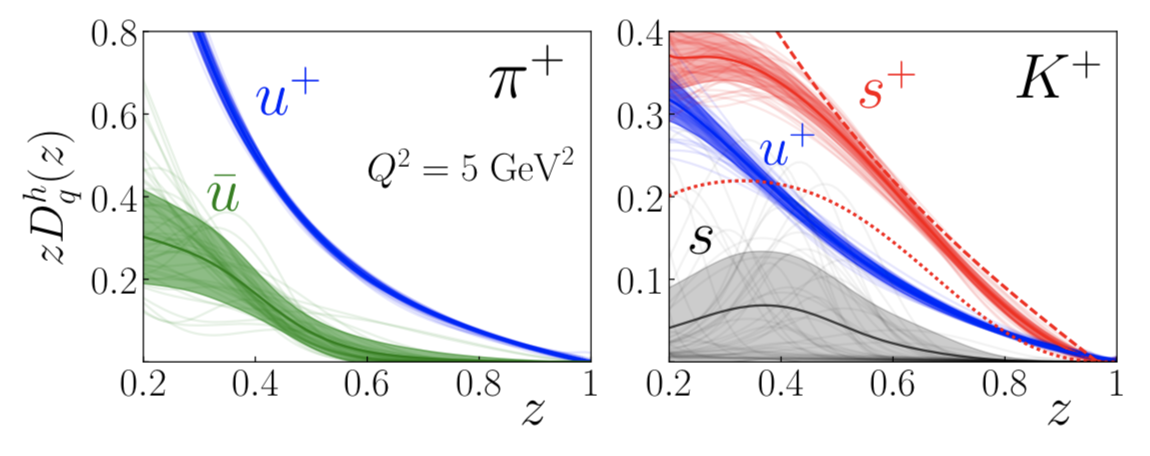
\includegraphics[scale=0.7]{./gfx/JAMcomp.png}
	\caption{Fragmentation functions $zD^h_q$ to $\pi^+$ (left panel) and $K^+$ (right panel) for $u^+$ (blue), $\bar{u}$ (green), $s^+$ (red) and $s$ (grey) at $Q^2$ = $5$ GeV$^2$ for the JAM$17$ analysis, compared to $s^+ \rightarrow K^+$ from DSS$07$ (dashed line) and HKNS (point line). Figure taken from \cite{JAM}.}
	\label{pic:JAMcomp}
\end{figure}

\section{Summary}

The DIS process is a very interesting channel for the study of the nucleon structure. The spin averaged PDFs, mostly determined from inclusive DIS, are well constrained in a wide kinematic domain for the first generation of quarks. Going to higher masses, large uncertainties still subsist e.g. for $s$ and $\bar{s}$. In SIDIS one gets additional access to FFs, which are universal quantities and parametrize quark hadronization.

Several groups have already issued parametrization of quark FFs based on LO and NLO analyses of various data sets. They differ significantly in the strange quark sector. This is why COMPASS did a new measurement and why the analysis presented in this was done.
